%!TEX root = ..\..\..\Main.tex
\section{Fourier Transform}

Reading from a devices sensors is done by taking samples of a signal at a certain frequency.
These samples estimate a wave which can be described as the sum of one or several sinusoids.
This wave is a function of time.
A Fourier Transforms task is to decompose this wave, and therefore the signal, into the frequencies of which it consists.
It can therefore be said that the Fourier Transform takes a signal from time domain, and converts it to frequency domain.

The maximum frequency resolution of a Fourier Transform is half the sampling rate, as per the Nyquist–Shannon sampling theorem.\cite{Digital_Signalbehandling}

The EEG's sample rate is 128Hz meaning the maximum resolution of any Fourier Transform applied to this signal would be 64Hz.

As an example, figure \ref{[FFT] Sample Signal} shows a generated signal consisting of a 50Hz sinusoid, a 120Hz sinusoid and some random whitenoise. The samplerate is 360Hz.
Passing this singal through a FFT (Fast Fourier Transform), it gives us the result shown in figure \ref{[FFT] Sample Result} which clearly shows spikes at x = 50 and x = 120, indicating the presence of a 50Hz and 120Hz sinusoid. \todomichael{Update these graphs. Also remember that the axes have to be labeled.}

\begin{figure}[h!]
  \centering
    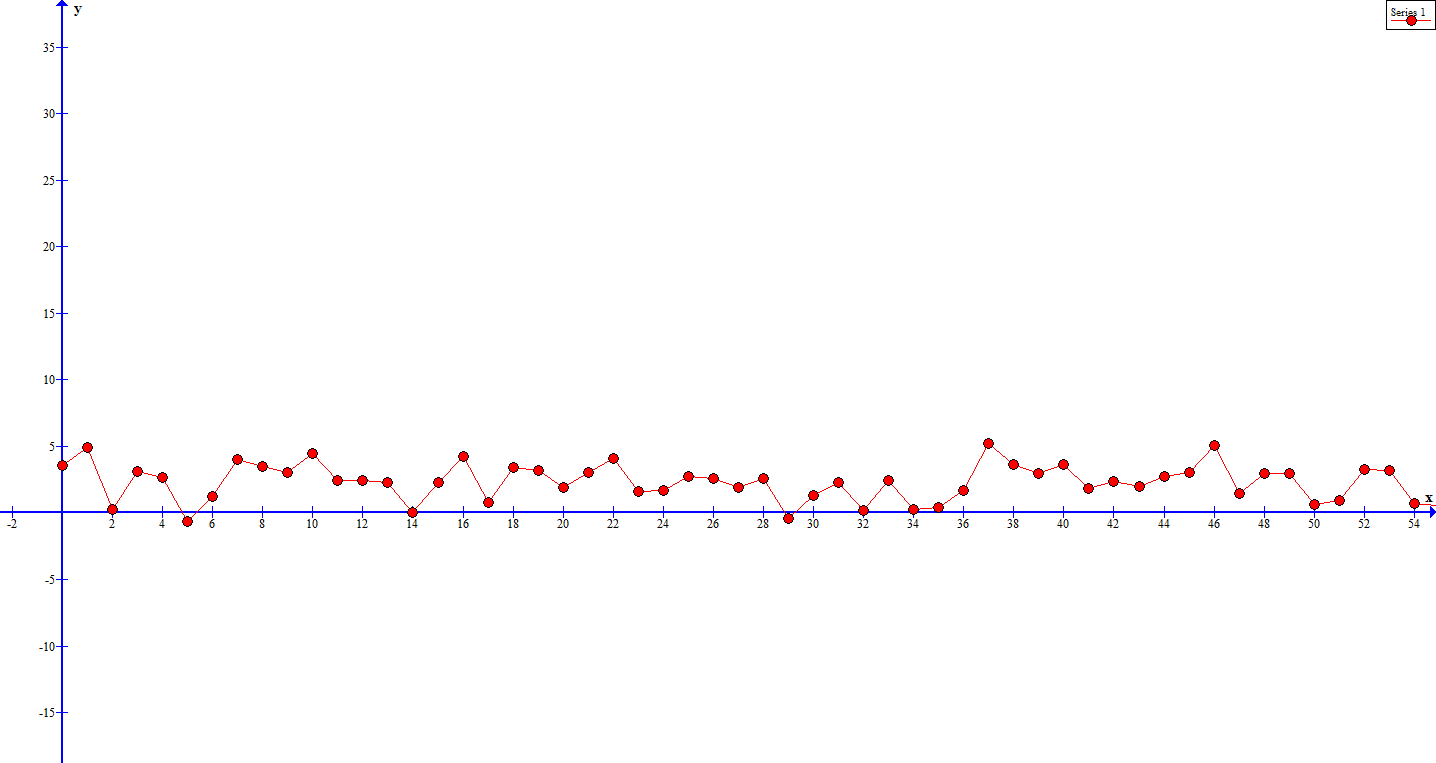
\includegraphics[width=1\textwidth]{sections/analysis/FFT/SampleCutout}
  \caption{Part of the generated signal.}
  \label{[FFT] Sample Signal}
\end{figure}

\begin{figure}[h!]
  \centering
    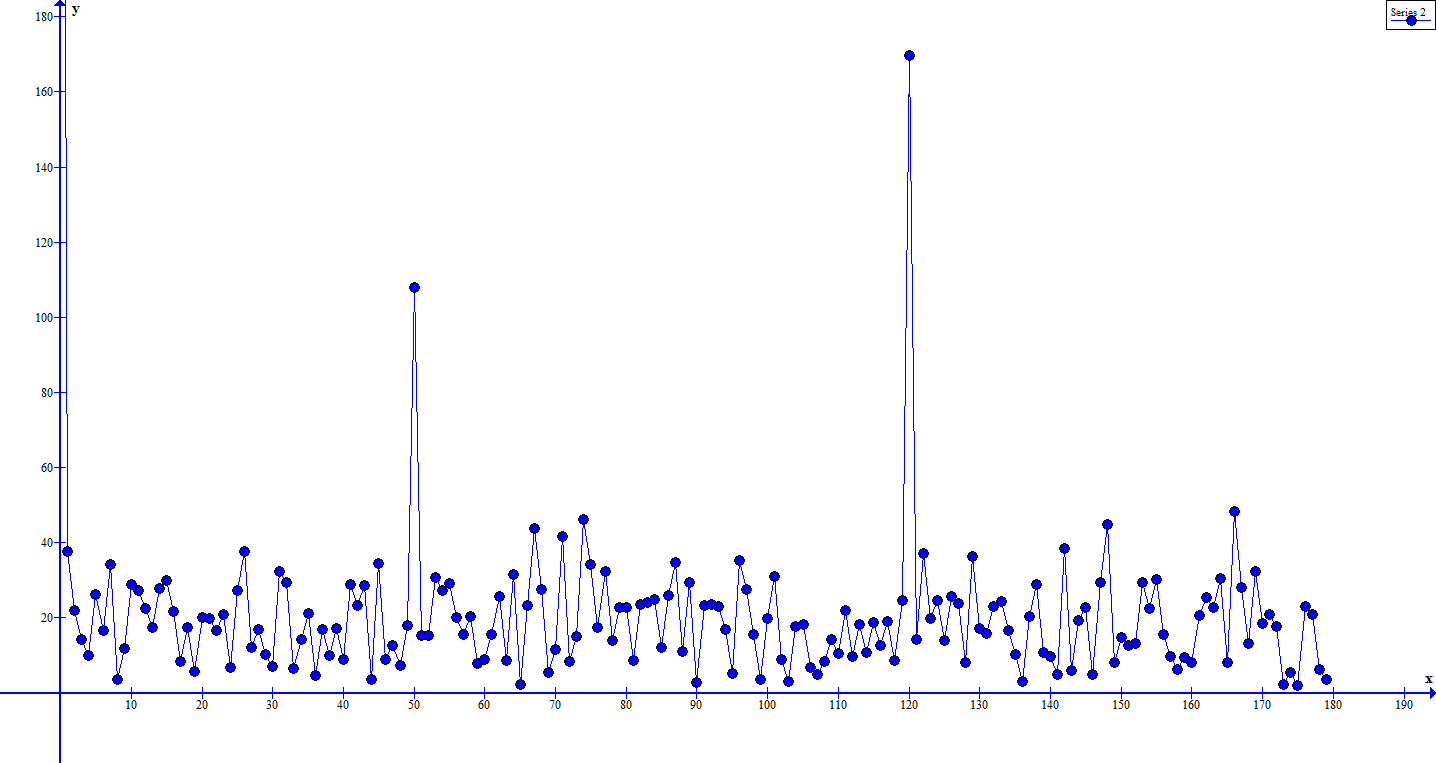
\includegraphics[width=1\textwidth]{sections/analysis/FFT/FFTResult}
  \caption{A FFT of the signal in figure \ref{SampleSignal}.}
  \label{[FFT] Sample Result}
\end{figure}